\chapter{Cameras}
\section{Network configuration}
There are two catecories of network configurations that needs to be done for the sensor platform to operate.



\subsection{IP configuration}
The \jx has a built in etherned adapter and the one osed on the \sr has been equipped with an extra wifi adapter, as well as a network card consisting of four independant ethernet adapters \cite{martensPortableSensorRig2022}.
The following section describes the different network configurations necessary to connect and communicate with the cameras. First two essential concepts are explained, then a IP configuration setup used to automatically detect the cammeras and assign IP adresses is presented.


\subsubsection{Reverse Path Filtering}
\gls{rpf} is a security feature that is designed to prevent IP address spoofing attacks by discarding incoming network traffic that does not have a valid return path \cite{ReversePathFiltering}.
However, in some cases, such as when discovering cameras over \gls{gigev} using \gls{lla}, disabling \gls{rpf} may be necessary ensure detection \cite{lucidvisionlabsArenaSoftwareDevelopment2020}. This can for example occur if the cameras IP address collides with that of the network adapter \cite{lucidvisionlabsArenaSoftwareDevelopment2020}. The followinc command can be used to disable \gls{rpf} \code{sudo sysctl -w net.ipv4.conf.eth1.rp_filter=0}.

\subsubsection{Link-Local Adress}
% In computer networking, \gls{lla} refers to an IP address that is used for communication within a logical division or broadcast domain to which the host is connected \cite{annieahujaweb2020LinkLocalAddress2022}.
% \gls{lla} is unique within a network segment, but not across different network segments, and therefore should not be forwarded by routers, this is however not relevant for this application \cite{annieahujaweb2020LinkLocalAddress2022}.
\gls{lla} is a method of IP address assignment that is often used when working with \gls{gigev} cameras \cite{teledyneSettingIPAddress01} \cite{lucidvisionlabsArenaSoftwareDevelopment2020}.
It allows devices to automatically assign IP addresses without the need for a \gls{dhcp} server or static IP \cite{annieahujaweb2020LinkLocalAddress2022}, which makes it possible to connect a \gls{gigev} camera directly to an ethernet adapter, without the need for an intermediate router.
For this to work properly the network adapter shoud be assigned the IP \code{169.254.0.1} and have netmask \code{255.255.0.0} as \gls{lla} addresses are assigned within the scope of \code{169.254.1.0} to \code{169.254.254.255} \cite{annieahujaweb2020LinkLocalAddress2022}\cite{lucidvisionlabsArenaSoftwareDevelopment2020}.

\subsubsection{Static IP}
A static IP address is one that is set up manually on a device, rather than being allocated by a DHCP server. It is referred to as static since it remains constant, in contrast to a dynamic IP address that can vary. \cite{fisherStaticIPAddresses2021}.
For \gls{gigev} Cameras using statid IP might be usefull as the cameras will power up with the same IP every time \cite{teledyneSettingPersistentIP}.

However I decided not to use static IP for the sensor rig setup, as it requiered the camera to be connected to the same ethernet port every time.
If the static IP of a camera was outside the IP range (\todo) of the network adapter it was connected to, or the network adapters had ovelapping IP ranges, the discovery process and connection got unstable.
Thus, to change which ethernet port a camera was connected to it would be necessary to either change the static IP of the camera, a tedious process, or change the IP range of both the current and previous ethernet adaptor.
An additional rationale for avoiding the use of static IP addresses is to keep the cameras' static configurations (the ones that persists when power cycling) the same as facory default.
This facilitates the use of the same cameras for a different project by someone else in the future.

\subsubsection{IP configuration Pipeline}


The discovery and enumeration process of the \lucid cameras is outlined in Figure \ref{fig:lucid_ip_discovery}.
\subsection{Network Performance}

\subsubsection{Jumbo Frames}
An Ethernet frame is a unit of packetized formatted information that includes the Ethernet header, payload, and CRC trailer. \cite{winterCisco3ComApplied2009}.
The original Ethernet specification, IEEE 802.3 \cite{ieeeIEEEStandardsInterpretation2002}, allowed for a frame size between 64 to 1518 bytes, with a standard header length of 18 bytes.
Ethernet Jumbo frames carry more payload than the maximum specified by IEEE 802.3, with an \gls{mtu} size of up to 9000 bytes \cite{lucidvisionlabsJumboFramesLUCID2020}.
Increasing the maximal \gls{mtu} size typically leads to improved performance for high-bandwidth cameras and can also help reduce the CPU load on the host system \cite{lucidvisionlabsJumboFramesLUCID2020}, as there is less protocol overhead \cite{lukeThingsYouShould2018}.
Both the ethernet card used on the \jx as well as the \cams support Jumbo frames \cite{IntelI350am4Chipa} \cite{TritonMPPolarized2020a}. To enable jumbo frames on a device (\code{eth1}) the following command is used \code{ifconfig eth1 mtu 9000}.

\subsubsection{Receive Buffers}
\begin{figure}
    \centering
    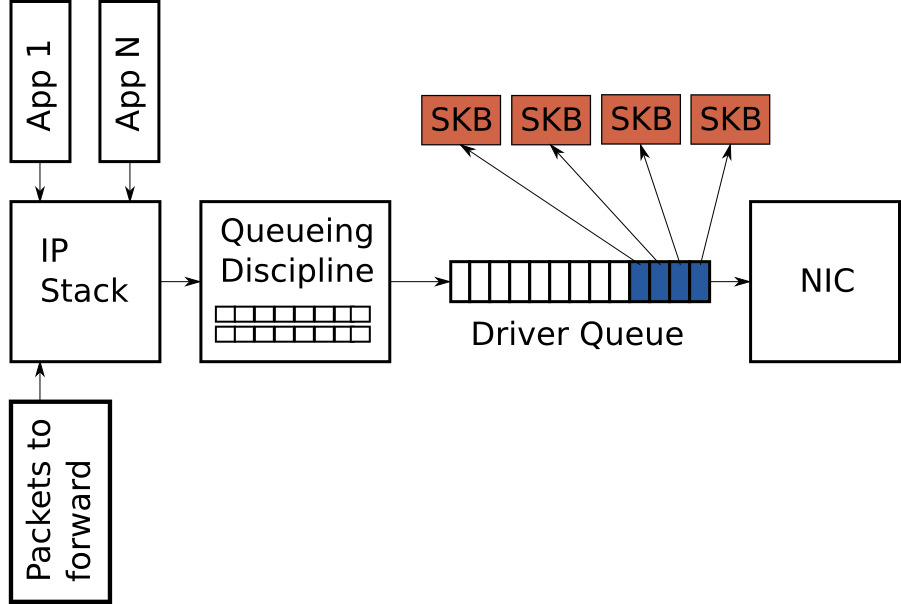
\includegraphics[width=0.8\textwidth]{figures/linux_networking.png}
    \caption{Simplified high level overview of the queues on the transmit path of the Linux network stack \cite{danQueueingLinuxNetwork2013}}
    \label{fig:linux_network}
\end{figure}
When network packets arrive on Linux they are stored in a driver queue as shown in Figure \ref{fig:linux_network} \cite{danQueueingLinuxNetwork2013}.
To avoid starvation and increase performance, it is recommended to increase the default number of \glspl{skb}, also known as receive buffers \cite{lucidvisionlabsReceiveBuffers2020} \cite{danQueueingLinuxNetwork2013}.
This can be done using the \mintinline{bash}{ethtool -G} command \cite{danQueueingLinuxNetwork2013}.
The maximal allowed number of receive buffers on the \jx are 4096, opposed to the default value of 256, according to the \mintinline{bash}{ethtool -g eth1} command.
The poetntial downside of increasing the number of \glspl{skb} is that it increases the memory usage and it might introduce more Latency as the Driver Queue gets longer \cite{danQueueingLinuxNetwork2013}. As the current use case for the sensor platform is to record data, this is not a problem, but it should be kept in mind for future work if the sensor platform is used for real-time applications.

As we are receiving large amounts of data as jumbo frames it is also recommended to increase the default and the maximal socket buffer size.
The default values for the default and maximal receive buffer saize were \todo and \todo, which was found using the \mintinline{bash}{sysctl -a | grep rmem_default} and \mintinline{bash}{sysctl -a | grep rmem_max} commands on a newly booted \jx \cite{sainiUnableReadNet2021}.

\lucid suggests setting both default and max buffer size to $1MiB$ while IBM suggest setting them up to $16MB$ for best performance \cite{lucidvisionlabsReceiveBuffers2020}\cite{ibmIBMDocumentationTCPIP2021}.
As it is quite cumbersome to perform low level network latency analysis, and memory depletion never seemed to be an issue with the $16GB$ of \gls{ram} available on the \jx, both default and max buffer size was set to $16MiB$.
To make this change permanent the following command is used \cite{redhat10ChangingNetwork}.
\begin{minted}{bash}
    $ sudo sh -c "echo 'net.core.rmem_default=16777216' >> /etc/sysctl.conf"
    $ sudo sh -c "echo 'net.core.rmem_max=16777216' >> /etc/sysctl.conf"
    $ sudo sysctl -p
\end{minted}







\begin{figure*}
    \centering
    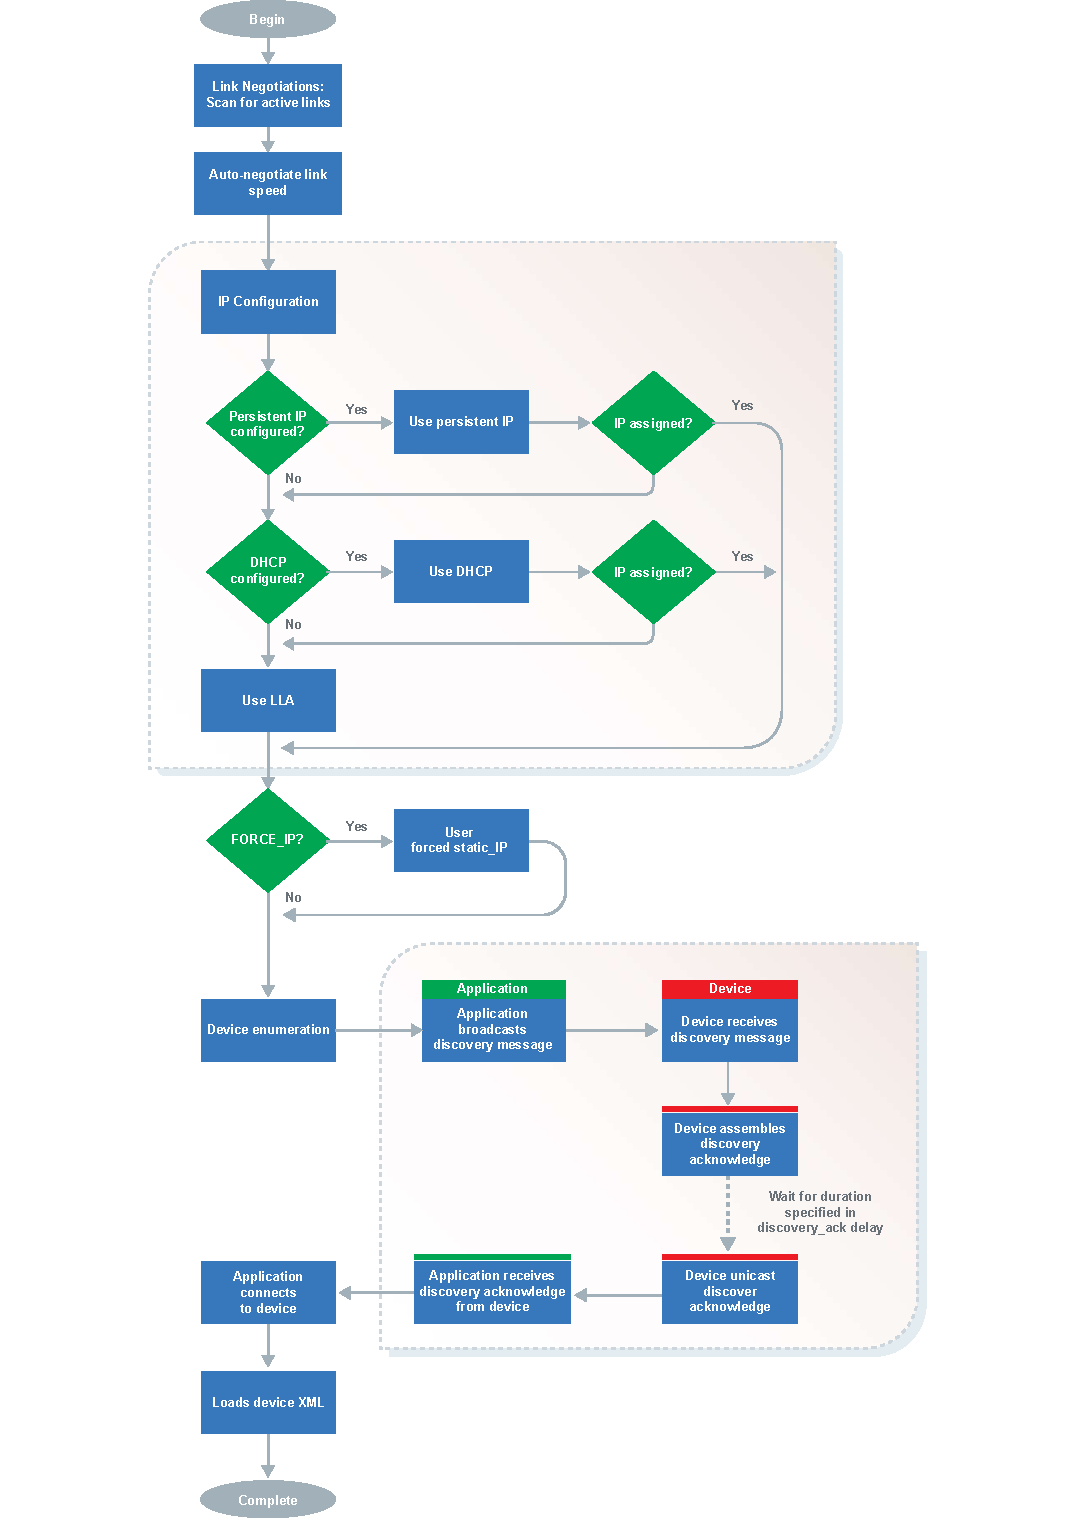
\includegraphics[height=\textheight]{figures/thing.pdf}
    \caption{Figure of the descovery and enumeration process of Lucid cameras \cite{TritonMPPolarized2020}}
    \label{fig:lucid_ip_discovery}
\end{figure*}

\section{Synchronization (PPT+PPS)}
Fast mode \approx $50\mu s$. Accurate mode prohibits $20hz$ refresh rate.
Verified using oscilloscope and analog output.
Cameras report ptp offset, but without a proper oscilloscope it is hard to verify if this is correct.


\section{Real time image processing}
Asyncio, subprocessing, queues and a lot of pain.



\section{Calibration}


\section{Network management}

Using network card.
A lot of configuration has to be done -> Python script.
\subsection*{Network card}
\subsection*{Jumbo Frames}
\subsection*{Receive Buffers}
\subsection*{Ip Address Assignment}
Local network for each eth device.
Assure no overlap.
\subsection*{LLA}
\subsection*{Reverse Path Filtering}



\section{Compression}
H265 for video, JPEG for images.
\subsection*{gstreamer}
\subsection*{Hardware acceleration}
Verified with \gls{jtop}.

\section{Custom debayering (GPU?)}
Not needed for now, but could be useful for future work.
Currently using OpenCV debayering.

An idea is to combine debayering, I420 conversion and polarization representations into one kernel.

\section{Polarization stuff}
Save all 4 polarization channels.
Gives more options for postprocessing in cases of ie saturation.

\section{Testing and verification of the system?}
Check compression loss.

\subsubsection{Receive Buffers}
\begin{figure}
    \centering
    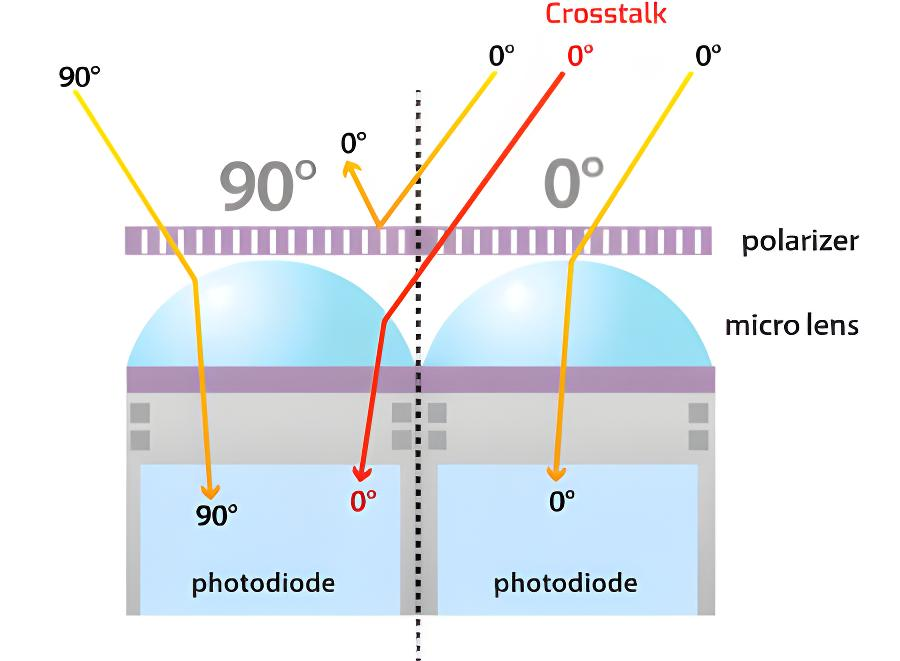
\includegraphics[width=0.8\textwidth]{figures/crosstalk_upscaled.jpg}
    \caption{$0^{\circ}$ polarized light is entering the pixel meant to detect $90^{\circ}$ and will be incorrectly detected as $90^{\circ}$.  This crosstalk error happens because the polarization array is placed above the micro lens \cite{lucidvisionlabsPolarizationExplainedSony2018}}
    \label{fig:camera_crosstalk}
\end{figure}
% \end{figure}
\begin{figure}
    \centering
    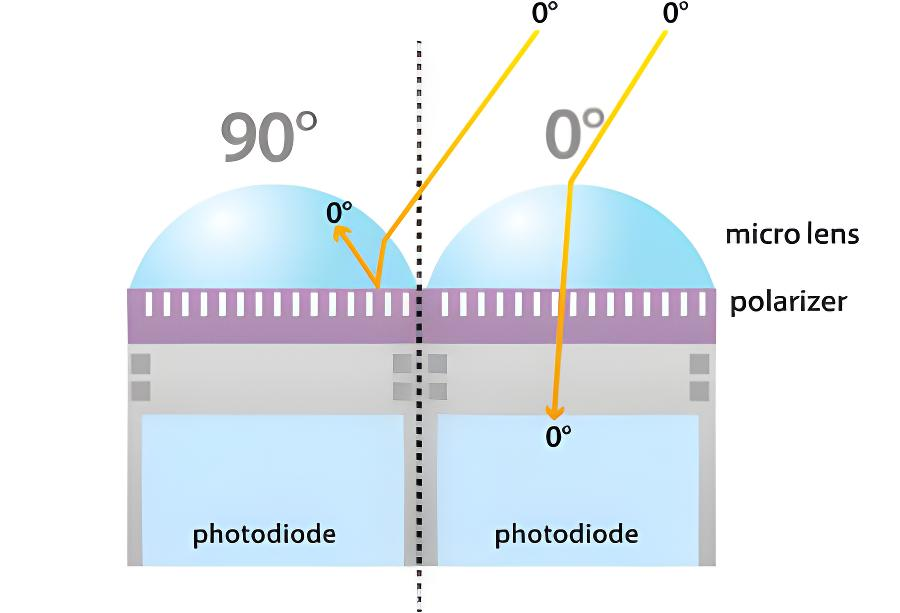
\includegraphics[width=0.8\textwidth]{figures/crosstalk_off_upscaled.jpg}
    \caption{Sony's polarization sensor reduces the chance of crosstalk thanks to the polarizer array being placed on-chip. The $0^{\circ}$ polarized light is unable to enter the pixel meant to detect only $90^{\circ}$ \cite{lucidvisionlabsPolarizationExplainedSony2018}}
    \label{fig:camera_no_crosstalk}
\end{figure}
